
\chapter{Data and Methodology}\label{ch:data_and_methodology}

This chapter describes the datasets, feature engineering pipeline, detrending methodology, rule-learning algorithms, walk-forward validation protocol, baseline models, and evaluation metrics used throughout the thesis. Section~\ref{sec:rulelearning_algorithms} provides a detailed technical description of all three rule-learning algorithms, including their internal mechanics, how they differ from one another, and why those differences matter for interpreting the results in Chapters~\ref{ch:goal_1_rule_extraction} and~\ref{ch:goal_2_predictive_performance}.


\section{Study Regions and Data}\label{sec:study_regions_and_data}

This study examines two geographically and climatically distinct Portuguese wine regions: the Douro Demarcated Region (RDD) and the Vinho Verde Region (RVV). The RDD dataset covers 89 annual observations from 1934 to 2022. The RVV dataset covers 80 annual observations from 1942 to 2021. Both datasets consist of one observation per year, where each observation contains a set of meteorological and phenological covariates together with annual wine production in thousands of hectolitres (mhl) as the response variable. Table~\ref{tab:ch3a_1} summarises the key characteristics of both datasets.

\begin{table}[htbp]
  \centering
  \caption{Dataset characteristics for the Douro (RDD) and Vinho Verde (RVV) study regions.}\label{tab:ch3a_1}
  \small
  \begin{adjustbox}{max width=\textwidth}
    \begin{tabularx}{\textwidth}{l|l|X}
  \toprule
  Characteristic & RDD (Douro) & RVV (Vinho Verde) \\
  \midrule
  Period & 1934--2022 & 1942--2021 \\
  Observations (n) & 89 years & 80 years \\
  Climate type & Continental / semi-arid & Temperate Atlantic \\
  Production trend & +80\% increase (1930s--2010s) & -65\% decline (1960s--2020s) \\
  Walk-forward scenarios & 18 & 16 \\
  Response variable & Annual wine production (mhl) & Annual wine production (mhl) \\
  \bottomrule
\end{tabularx}
  \end{adjustbox}

\end{table}




Because both series are non-stationary, random cross-validation is not appropriate; a walk-forward expanding-window protocol is used instead, as described in Section~\ref{sec:walkforward_validation_protocol}.

Figures~\ref{fig:context_ts_rdd} and~\ref{fig:context_ts_rvv} show the annual production time series for the two regions, illustrating the opposing structural trends summarised in Table~\ref{tab:ch3a_1}.

\begin{figure}[htbp]
  \centering
  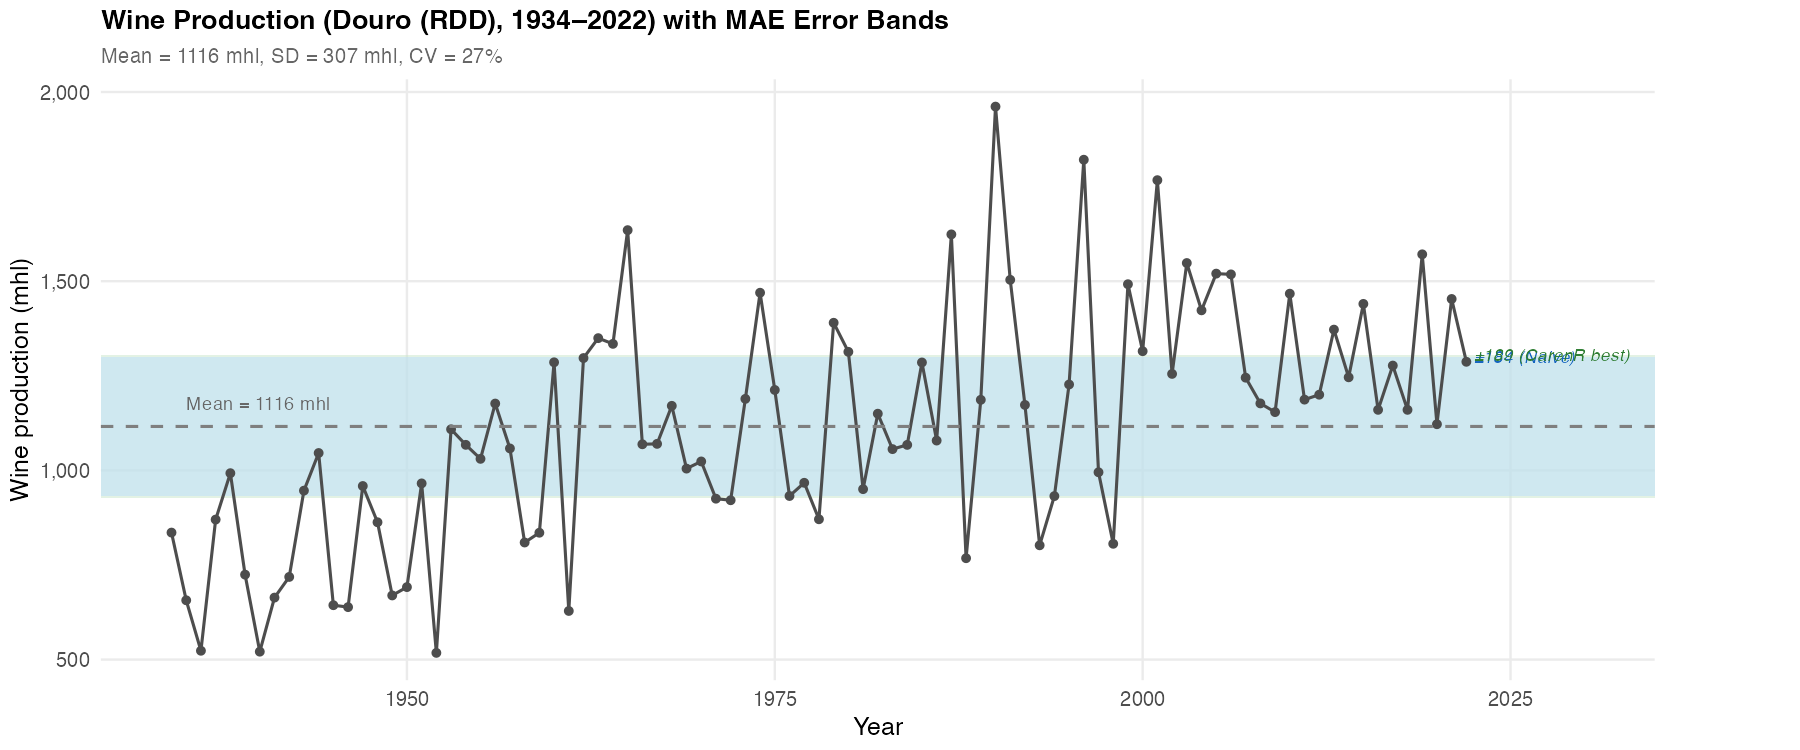
\includegraphics[width=0.85\textwidth]{figures/fig_context_ts_rdd.png}
  \caption{Production time series for the Douro (RDD) region, 1934--2022.}
  \label{fig:context_ts_rdd}
\end{figure}

\begin{figure}[htbp]
  \centering
  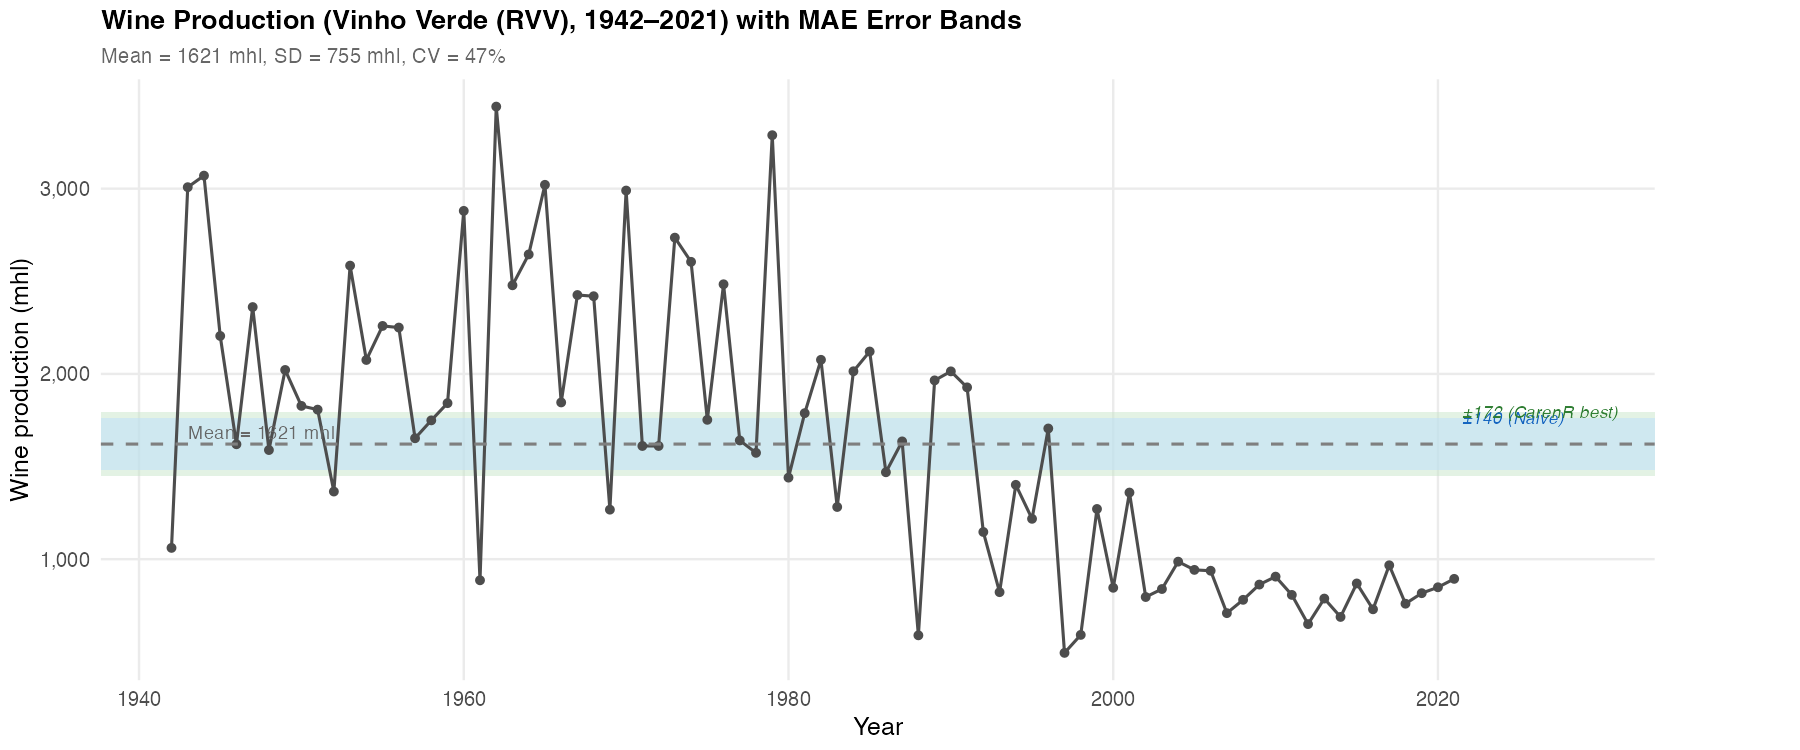
\includegraphics[width=0.85\textwidth]{figures/fig_context_ts_rvv.png}
  \caption{Production time series for the Vinho Verde (RVV) region, 1942--2021.}
  \label{fig:context_ts_rvv}
\end{figure}


\section{Feature Engineering}\label{sec:feature_engineering}

Covariates were constructed from daily temperature, rainfall, and soil water balance records, supplemented by Leaf Area Index (LAI) estimates from a vine phenological model. All variables were aggregated over windows defined by phenological stage and calendar date, producing features that correspond to agronomically meaningful periods of vine development. The feature naming convention encodes the variable type, phenological stage, year offset (current or previous year), and window width; for example, swa\_hv\_y1\_b20 denotes soil water availability (swa) in the 20 days before (b20) harvest (hv) in the current year (y1).

Feature families included: mean and minimum temperature at each phenological window; total rainfall and number of wet days (days with rainfall > 1 mm); soil water availability (mm) at budburst, flowering, veraison, and harvest; accumulated heat degree-days above 35$^\circ$C and cold days below 15$^\circ$C; and LAI at budburst and flowering. Lagged versions of selected features (previous growing season, denoted y0) were included to capture carryover effects from the prior year. The final feature matrix contained 59 candidate predictors per region.



\subsection{Autocorrelation Structure of the Residuals}\label{sub:autocorrelation_structure_of_the}

Before designing the previous-year (y0) features, the autocorrelation structure of the linearly detrended production residuals was examined to determine which lags carry statistically significant serial dependence. This analysis was performed on the target variable only --- not on the climate features. It served two purposes: (1) providing empirical confirmation that lag-1 production autocorrelation is negligible, supporting the use of climate features rather than lagged production values as predictors; and (2) revealing longer-period cyclical structure that motivated the \texttt{CarenR\_Dist\_Lag} variant (Section~\ref{sec:feature_selector_comparison_why}).

The ACF and PACF of the linearly detrended residuals (up to lag~12 years, 95\% confidence bands $\pm 1.96/\sqrt{n}$) show two key findings. \textbf{Lag~1 is not significant} in either region (RDD: ACF~$= +0.08$; RVV: ACF~$= +0.19$, both below the confidence threshold). This means that knowing last year's production does not reliably predict the current year's deviation from trend, directly explaining why the Naive ``last value'' baseline underperforms Naive\_Median (Table~\ref{tab:ch5a_1}: Naive 199~mhl vs.\ Naive\_Median 184~mhl for RDD). \textbf{Lags 5--6 are significant in both regions} (ACF at lag~5: $+0.22$ for RDD, $+0.30$ for RVV), consistent with the $\sim$5.7-year dominant production cycle identified by \citet{Cunha2020}. The \texttt{CarenR\_Dist\_Lag} variant was designed to exploit this cycle by augmenting the feature set with ACF-selected lagged residuals; it ranked 5th in RDD and 8th in RVV, suggesting the cycle is statistically present but does not translate into a reliably exploitable predictive signal relative to the domain-knowledge-based y0 features.

\section{Detrending and the Two-Decision Decomposition}\label{sec:detrending_and_the_twodecision}

All models operate on linearly detrended residuals $r_t = y_t - (\alpha + \beta t)$, where $y_t$ is observed production and $\alpha + \beta t$ is the OLS linear trend estimated on the training set. Predictions are converted back to the original scale by adding the projected trend value: $\hat{y}_t = r_t + (\alpha + \beta t)$. All preprocessing steps are performed exclusively on the training fold within each scenario to prevent data leakage.

\textbf{Decision 1 --- Trend modelling: }how accurately does the training-period trend extrapolate to test years? Measured by Naive\_Median MAE.

\textbf{Decision 2 --- Climate signal extraction: }can a rule-based model predict detrended residuals better than zero? Measured by the gap between a model's weighted MAE and the Naive\_Median weighted MAE.


\section{Rule-Learning Algorithms}\label{sec:rulelearning_algorithms}

Three rule-learning algorithms were evaluated, representing three fundamentally different approaches to extracting interpretable patterns from the same data. Understanding how each algorithm works internally, and specifically what question it is designed to answer, is essential for correctly interpreting the results in Chapter~\ref{ch:goal_1_rule_extraction} and the comparison in Section~\ref{sec:crossalgorithm_feature_agreement}. Table~\ref{tab:ch3a_2} summarises the key characteristics of all three algorithms before each is described in detail. The two bottom rows of the table describe not intrinsic properties of the algorithms but how each is operationalised for numeric forecasting within the prediction framework defined in this thesis.

\begin{table}[htbp]
  \centering
  \caption{Comparison of the three rule-learning algorithms: CarenR, RIPPER, and M5Rules.}\label{tab:ch3a_2}
  \small
  \begin{adjustbox}{max width=\textwidth}
    \begin{tabularx}{\textwidth}{>{\bfseries}p{3cm} X X X}
    \toprule
    Property & \textbf{CarenR} & \textbf{RIPPER} & \textbf{M5Rules} \\
    \midrule
    Task type
      & Distributional subgroup discovery
      & Classification rule learning
      & Piecewise linear regression \\[4pt]
    Target variable
      & Continuous (detrended residuals)
      & Discretised classes (Low / Med / High)
      & Continuous (detrended residuals) \\[4pt]
    Core question answered
      & When does the shape of the production distribution shift significantly?
      & Which climate class does a year belong to?
      & What exact production level does a year have? \\[4pt]
    Statistical criterion
      & Kolmogorov--Smirnov two-sample test ($p \leq 0.10$)
      & Information gain / Gini (FOIL gain for rule growing)
      & Standard deviation reduction (MSE minimisation) \\[4pt]
    Rule output
      & IF conditions THEN distribution shifts up / down
      & IF conditions THEN class = Low / Med / High
      & IF conditions THEN production = linear model(features) \\[4pt]
    Feature input
      & Discretised equal-frequency bins
      & Continuous (RIPPER finds own thresholds)
      & Continuous (M5Rules finds own thresholds) \\[4pt]
    Interpretability
      & Very high --- simple IF/THEN with distributional evidence
      & High --- ordered IF/THEN classification
      & Medium --- IF/THEN rules with linear models at leaves \\[4pt]
    \midrule
    \multicolumn{4}{l}{\normalfont\itshape Operationalisation for prediction in this thesis (Section~\ref{sub:prediction_aggregation_combining_multiple})} \\
    \midrule
    Prediction output
      & Mean/median of matching subgroup
      & Class midpoint or median
      & Linear model evaluated at feature values \\[4pt]
    Fallback (no rules fire)
      & Training median residual
      & Default rule (most common class)
      & Global linear model (no conditions) \\
    \bottomrule
  \end{tabularx}
  \end{adjustbox}

\end{table}



\subsection{CarenR: Distribution Rules via the CAREN Framework}\label{sub:carenr_distribution_rules_via}

CarenR is built on the CAREN association rule engine, originally developed by \citet{Jorge2006} for discovering distribution rules in numeric data. It is the primary algorithm of this thesis and the only one of the three that is specifically designed for continuous response variables without requiring pre-discretisation of the target. This section describes its mechanics in detail.

\textbf{Conceptual foundation. }Most rule-learning algorithms ask: ``what value does this observation have?'' CarenR asks a different question: ``is there a subgroup of observations, defined by a conjunction of input feature conditions, where the statistical distribution of the target variable is significantly different from the distribution across the full dataset?'' A CarenR rule does not say ``this year will produce X mhl.'' It says ``in years satisfying these climate conditions, the production distribution is shifted upward (or downward) in a statistically significant way, the entire distributional shape is different --- not just the mean.'' This distinction between point prediction and distributional shift is fundamental to understanding both the strengths and the limitations of CarenR.

\textbf{Step 1: Feature discretisation. }CarenR requires discrete (ordinal) input features. Each continuous climate feature is independently discretised into four equal-frequency bins (quartiles). Equal-frequency binning ensures that each bin contains approximately the same number of observations, avoiding sparse bins at extreme values that would make the KS test unreliable. For example, the feature swa\_hv\_y1\_b20 (soil water 20 days before harvest) might be discretised into bins [20--74 mm], [74--101 mm], [101--152 mm], [152--350 mm], each containing approximately 22 of the 89 RDD observations. For Goal 1 (Rule Discovery), bin boundaries are computed on the full historical dataset. For Goal 2 (Predictive Validation), bin boundaries are computed exclusively on the training fold within each scenario, preventing any leakage of test-set information into the discretisation step.

\textbf{Step 2: Feature selection (Goal 2 only). }This step applies only to Goal 2 (Predictive Validation). For Goal 1 (Rule Discovery), CarenR operates on all 59 domain-engineered features without further algorithmic filtering --- the feature set is defined entirely by viticulture domain knowledge. For Goal 2, with 59 candidate features each discretised into 4 bins, the full itemset search space is combinatorially large, and a feature selection step reduces the feature set before rule induction. This thesis evaluates several selection strategies (described in Table~\ref{tab:ch3a_3}) as distinct CarenR variants. Three selection strategies are evaluated, each reflecting a different way of measuring association between a discrete feature and a continuous target. $\eta$$^2$-based selection (eta-squared) is the most statistically appropriate: it applies a one-way ANOVA across the four bins of each feature and measures how much of the variance in the continuous production residual is explained by the discrete groupings --- directly answering whether the bins produce meaningfully different production distributions. Pearson correlation (|r| above the median across all features) is a simpler approximation that treats the bin numbers as equally spaced ordinal values; it is less rigorous but computationally efficient and tends to identify the same features in practice. Support-filtered Pearson selection adds a coverage requirement: each bin of a retained feature must contain at least a minimum fraction of training observations, preventing selection of features with extreme or sparse bin distributions. The convergence of all three strategies on the same variable families (confirmed in Section~\ref{sec:crossalgorithm_feature_agreement}) is evidence that the feature rankings are robust to the choice of selection criterion. All feature selection is performed exclusively on training data within each fold.

\textbf{Step 3: Rule induction via subgroup search. }CarenR searches for conjunctions of feature-bin conditions (itemsets) that define subgroups with distributional shift in the target variable. The search proceeds breadth-first: single-condition rules are evaluated first, then two-condition conjunctions are formed from the most promising single conditions, and so on up to a maximum rule length (typically 3--4 conditions). For each candidate subgroup, the observations satisfying all conditions are identified --- for Goal 1 this is the full historical dataset; for Goal 2 it is the training fold --- and a two-sample Kolmogorov--Smirnov (KS) test is performed comparing the target distribution in the subgroup against the global distribution.

\textbf{Step 4: The Kolmogorov--Smirnov test. }The KS test is a non-parametric statistical test that compares two empirical cumulative distribution functions (ECDFs). Given a subgroup $S$ of $n_S$ observations and the global reference set of $n_T$ observations (the full dataset for Goal 1, the training fold for Goal 2), the KS statistic $D$ is the maximum absolute difference between the two ECDFs:

\begin{equation}
  D = \max_{x} \left| F_S(x) - F_T(x) \right|
  \label{eq:ks}
\end{equation}

where $F_S(x)$ is the empirical CDF of the target in the subgroup and $F_T(x)$ is the empirical CDF in the global set. A large $D$ indicates that the two distributions are far apart --- the subgroup has a systematically different pattern of production values. The $p$-value associated with $D$ measures the probability of observing a difference of this magnitude by chance if the two samples were drawn from the same distribution. A rule is retained only if $p \leq 0.10$ (the significance threshold used in this study). The KS test makes no assumption about the shape of either distribution, which is important given the small sample sizes ($n = 80$--$89$) and the non-normal distribution of production residuals.

\textbf{Step 5: Support filter. }A statistically significant rule that covers only two or three observations (very low support) is not useful: it describes a pattern too rare to be actionable and is likely to be a chance finding. CarenR therefore applies a minimum support filter: a rule is retained only if it covers a minimum fraction of the reference observations. The threshold value is not prescribed by the algorithm but is an experimental design decision of this thesis: it was set to 15\% (Table~\ref{tab:ch3d_7}) --- approximately 12--13 years for an 89-year dataset in Goal 1, or the equivalent share of the training fold in Goal 2. This filter ensures that reported rules represent patterns that recur across a meaningful portion of the historical record rather than isolated individual years, improving their robustness and practical interpretability.

\textbf{Step 6: Rule output and prediction. }Each retained rule describes a climate subgroup as a conjunction of feature-bin conditions, along with the median residual of the target variable within the subgroup and the KS p-value. An example RDD rule output reads: ``IF wet days post-flowering $\in$ [0, 3.33] AND wet days post-maturity $\in$ [0, 3.46] THEN production is +121 mhl above trend on average (support 28\%, p = 0.0043).'' For Goal 1, the retained rules are the direct output --- each rule represents an interpretable agroclimatic pattern. For Goal 2 (Predictive Validation), the feature values of a test year are checked against all retained rules. If one or more rules fire, their subgroup medians are combined as a support-weighted average --- each rule's median residual weighted by its support fraction, with weights normalised to sum to one. If no rule fires, the model falls back to the training median residual, producing the same prediction as the Naive\_Median baseline. This fallback means CarenR never predicts worse than the naive baseline unless it fires a rule, which makes the walk-forward evaluation in Chapter~\ref{ch:goal_2_predictive_performance} a direct test of whether the fired rules add value beyond the median.

\textbf{What makes CarenR unique. }Figure~\ref{fig:ch3_carenr_flow} illustrates the full CarenR pipeline including the thesis-level design choices. Three properties distinguish CarenR from standard rule learners. First, the KS-test criterion detects distributional shift rather than class membership or squared error reduction. This allows CarenR to identify features whose relationship with production is probabilistic and distributional, for example, LAI at harvest in Vinho Verde (Section~\ref{sub:vinho_verde_rvv_feature}), which reliably shifts the distribution of production residuals without reliably predicting any single year's exact value. Second, rules are verified against a global null distribution rather than constructed greedily to separate pre-defined classes, making them statistically grounded in a way that classification rules are not. Third, the prediction framework developed in this thesis incorporates an explicit fallback mechanism: when no rule matches a test year's conditions, the prediction defaults to the training median rather than forcing an uninformed estimate. This design choice makes the overall approach conservative --- it only departs from the naive baseline when at least one rule fires, ensuring that CarenR's predictions can only add noise if they are wrong, never if they abstain.


\begin{figure}[!ht]
  \centering
  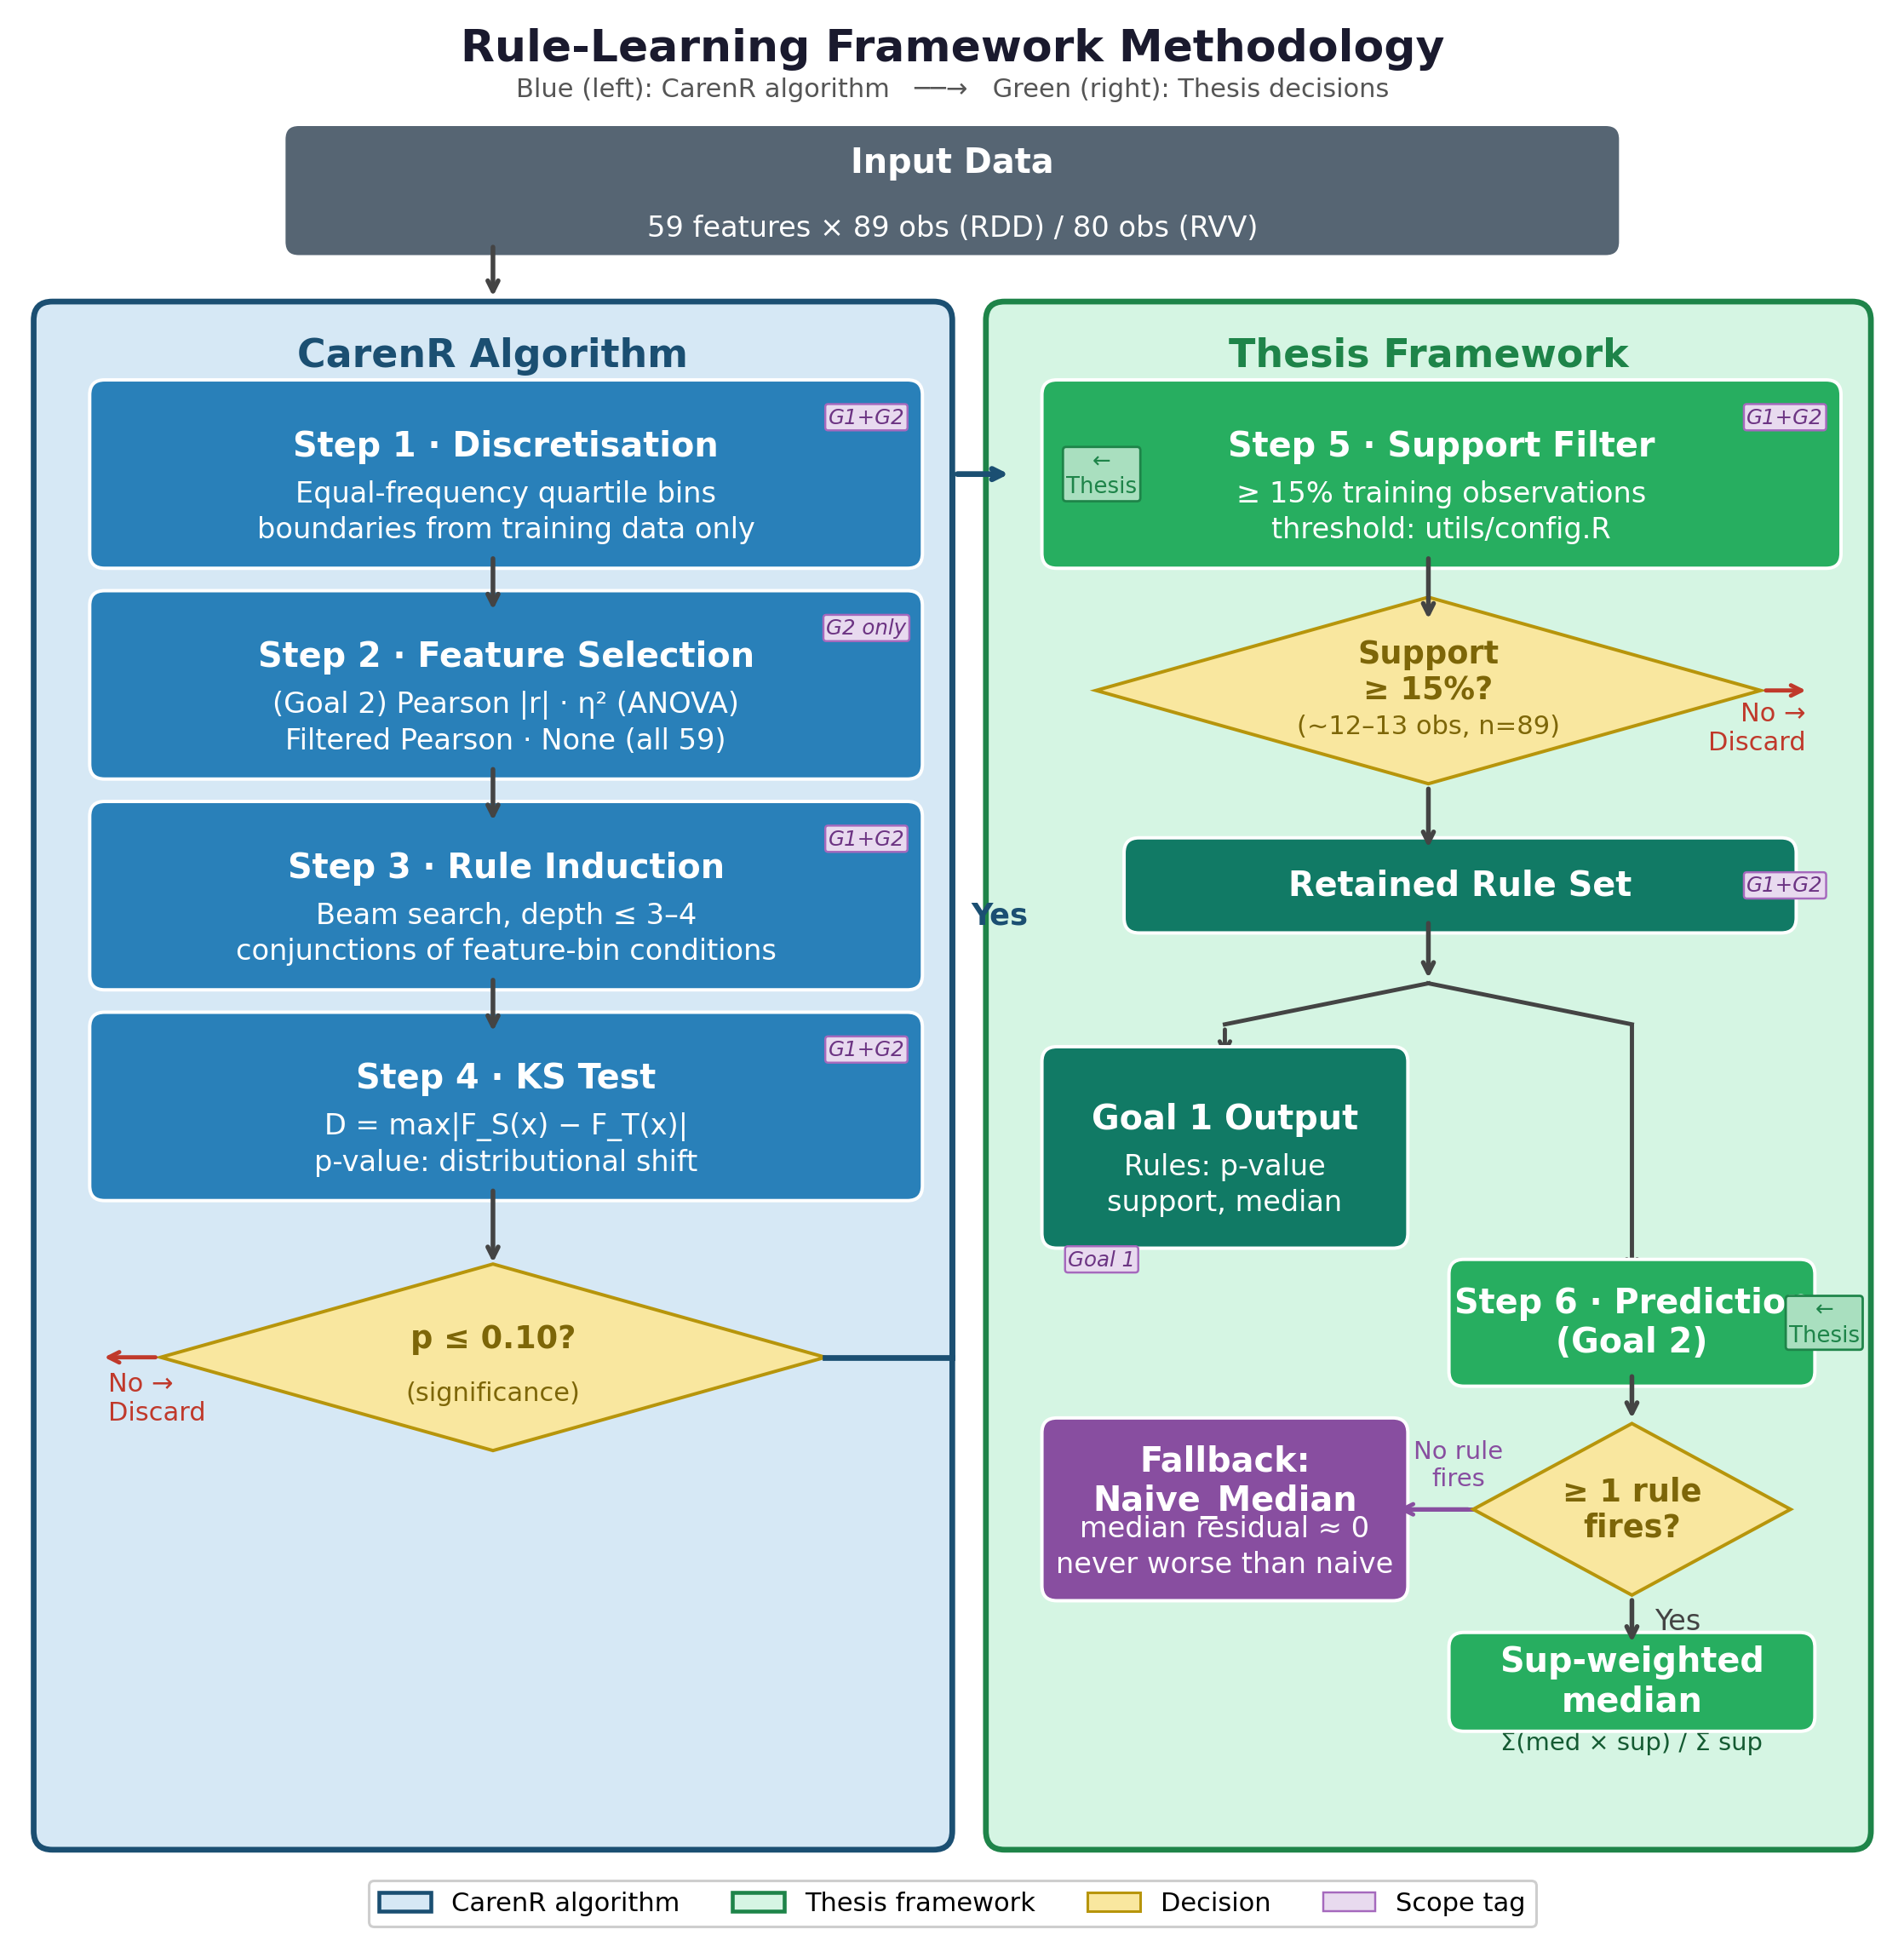
\includegraphics[width=\textwidth]{figures/fig_ch3_carenr_flowchart.png}
  \caption{Rule-learning framework methodology: CarenR algorithm steps (blue, left) and thesis framework decisions (green, right). The significance threshold, support filter, prediction logic, and fallback are thesis design choices, not prescribed by the CarenR algorithm.}
  \label{fig:ch3_carenr_flow}
\end{figure}


\subsection{RIPPER: Repeated Incremental Pruning to Produce Error Reduction}\label{sub:ripper_repeated_incremental_pruning}

RIPPER, implemented as JRip in the Weka machine learning toolkit \citep{Witten2011}, is a propositional rule learning algorithm for classification. It was introduced by \citet{Cohen1995} as an efficient, scalable alternative to earlier rule learners such as CN2, and remains one of the most widely used interpretable classification algorithms. In this thesis RIPPER serves as an interpretable classification benchmark, allowing the rules found by CarenR to be compared against a well-established rule-based classification baseline.

\textbf{Target discretisation. }RIPPER is a classifier and requires a discrete target variable. The continuous production residuals are therefore discretised into three ordinal classes --- Low, Medium, and High --- using tertile boundaries. For Goal 1 (Rule Discovery), boundaries are estimated on the full historical dataset. For Goal 2 (Predictive Validation), boundaries are estimated within each training fold to prevent leakage. Each class contains approximately one third of the observations. This discretisation step introduces a loss of information relative to CarenR and M5Rules, which both operate on the continuous response.

\textbf{Rule growing with FOIL gain. }RIPPER constructs rules one class at a time, starting with the minority class and working towards the majority class. For each class, it grows a rule by greedily adding conditions that maximise the FOIL information gain, a measure that rewards conditions that increase the ratio of positive (target class) to negative (other class) examples covered by the rule. Starting from an empty condition set, RIPPER adds one condition at a time until no further gain is possible or a stopping criterion is met. The grown rule is typically a conjunction of 2--5 conditions that together define a subregion of feature space highly concentrated in the target class.

For a rule $R$ and candidate extension $R'$ (adding one condition), the FOIL gain is:
\begin{equation}
  \text{FOIL-gain}(R, R') = p' \left(\log_2\frac{p'}{p'+n'} - \log_2\frac{p}{p+n}\right)
  \label{eq:foil}
\end{equation}
where $p$ and $n$ are the numbers of positive and negative examples covered by $R$, and $p'$, $n'$ are the corresponding counts for the extended rule $R'$. RIPPER selects the condition $c^* = \arg\max_c \,\text{FOIL-gain}(R, R \cup \{c\})$ at each growing step.

\textbf{Rule pruning with MDL. }Overfitting is controlled by a pruning step that removes conditions from the grown rule using the Minimum Description Length (MDL) principle: conditions whose removal reduces the total description length of the rule set plus the data are deleted. This balances rule complexity against coverage, a rule that is slightly less precise but covers more observations is preferred over a highly specific rule covering very few. After pruning, RIPPER checks whether replacing or revising a rule reduces the total error, iterating until convergence. Note that RIPPER's internal pruning mechanism uses an internal hold-out fraction of the training data (not random cross-validation across the full dataset), so it does not violate the temporal ordering enforced by the walk-forward protocol: the internal hold-out is drawn from the same training fold already bounded by the current scenario's cut-point.

\textbf{Ordered rule list and default rule. }The final output of RIPPER is an ordered rule list: rules are applied in the order they were learned, and the first rule whose conditions are satisfied assigns the class for a given observation. Any observation not covered by any explicit rule is assigned the default class, the most frequent class in the training data. This ordered, default-inclusive structure ensures complete coverage: every observation receives a class label. In this thesis, the default rule covered the majority of observations (all years not matching explicit climate conditions), limiting RIPPER's ability to characterise positive (above-trend) production years in the Douro.

\textbf{Why RIPPER struggles with small datasets. }RIPPER was designed for large databases where each class is represented by thousands of examples. With n = 80--89 observations split into three classes of approximately 27--30 each, the per-class sample size is very small relative to the dimensionality of the feature space. FOIL gain estimates are unreliable on such small samples, and the MDL pruning criterion may be too aggressive or too permissive. The result is either overly specific rules (high precision, very low support) or a near-trivial rule list (one or two rules plus a default) that captures only the most obvious patterns. Cross-validated accuracy of 35--42\%, only slightly above the 33\% random baseline, reflects this limitation directly.


\subsection{M5Rules: Rule Induction with Linear Regression Consequents}\label{sub:m5rules_rule_induction_with}

M5Rules, also implemented in Weka, is a piecewise linear regression rule learner derived from the M5 model tree algorithm \citep{Quinlan1992,Wang1997}. Instead of predicting a class label or a distributional shift, M5Rules predicts an exact numerical value for each observation by applying a linear regression model whose coefficients depend on which region of feature space the observation falls in. This makes M5Rules the only algorithm in this study that produces a direct point estimate of the production residual, making it directly comparable to the naive baseline and to CarenR's subgroup-median prediction.

\textbf{Model tree construction. }M5Rules begins by constructing a regression model tree using a top-down recursive partitioning procedure. At each node of the tree, M5Rules selects the feature and split threshold that maximise the reduction in standard deviation of the target variable across the two resulting child nodes, analogous to the variance reduction criterion used by CART, but applied to a regression setting. This process continues recursively until each leaf contains a minimum number of observations (default: 4 in Weka). The result is a binary tree that partitions the feature space into disjoint regions, with a multivariate linear regression model estimated at each leaf using the observations that reach it.

The standard deviation reduction (SDR) for a split of training set $T$ into subsets $T_L$ and $T_R$ is:
\begin{equation}
  \text{SDR}(T, T_L, T_R) = \text{sd}(T) - \frac{|T_L|}{|T|}\,\text{sd}(T_L) - \frac{|T_R|}{|T|}\,\text{sd}(T_R)
  \label{eq:sdr}
\end{equation}
where $\text{sd}(\cdot)$ denotes the sample standard deviation of the response variable in the corresponding set.

\textbf{Leaf model estimation and smoothing. }Within each leaf, a linear regression model is fitted to the training observations in that leaf using ordinary least squares. M5Rules applies a smoothing procedure that interpolates between the leaf model and progressively coarser ancestor models as the observation moves up the tree, reducing the discontinuities at split boundaries that would otherwise produce implausible predictions near the edges of each leaf region. The smoothed prediction at leaf depth d is a weighted combination of the leaf model and each ancestor model's prediction.

\textbf{Pruning and conversion to rules. }After tree construction, M5Rules prunes branches whose removal does not increase cross-validation error beyond a tolerance threshold. The pruned tree is then converted into an ordered rule list: each path from the root to a leaf becomes one rule, with the conditions along the path as the antecedent and the leaf's linear model as the consequent. Rules are applied in order; the first matching rule is used, with the final rule having no conditions (applies to all observations) as a universal default. This conversion gives M5Rules the same human-readable rule format as RIPPER but with a linear model at each leaf rather than a class label.

\textbf{Why M5Rules collapses to a global model on small datasets. }M5Rules' standard deviation reduction criterion requires that each split create two child nodes, each with sufficient observations for reliable linear regression. With a minimum leaf size of 4 and n = 80--89 training observations, the algorithm cannot split the data more than a few times before individual leaves become too small for stable regression. In practice, M5Rules found no beneficial split in either region on the full dataset, collapsing to a single global linear model: one rule with no conditions that applies to all observations. This global model fits the training data with R$^2$ $\approx$ 0.40--0.53 but generalises poorly, with cross-validated R$^2$ falling to 0.004 (RDD) and -0.07 (RVV). The negative CV R$^2$ for RVV confirms that the model is worse than simply predicting the global mean; it has overfit the training set despite using a single linear equation.

\textbf{Comparison with CarenR and RIPPER. }The three algorithms differ fundamentally in what they optimise and what they produce. CarenR searches for distributional anomalies using a non-parametric test; it will find a feature informative if it shifts the distribution of production residuals in a statistically reliable way, even if that shift is not captured by a linear coefficient or a class boundary. RIPPER searches for class-separating conditions using information gain; it will find a feature informative if it concentrates one production class, regardless of the distribution of other classes. M5Rules searches for variance-reducing splits using squared error; it will find a feature informative if it enables a more accurate linear model, penalising large deviations quadratically. A feature that shifts the mean of the distribution of production residuals (detected by CarenR) but does not cleanly separate the three classes (not detected by RIPPER) and adds noise rather than linearity to the regression (not detected by M5Rules) will appear in CarenR's output but not in the others. This is precisely the situation for LAI at harvest in Vinho Verde, as discussed in Section~\ref{sub:vinho_verde_rvv_feature}.


\section{Walk-Forward Validation Protocol}\label{sec:walkforward_validation_protocol}

Model performance for Goal 2 was assessed using a walk-forward expanding-window validation, illustrated in Figure~\ref{fig:ch3_walkforward}. The earliest 80\% of each regional time series defines the minimum training window. At each subsequent step (scenario), the training window is extended by one year and the model is re-fitted from scratch on all available training data; the next year is then predicted and its prediction error recorded. This generates 18 evaluation scenarios for RDD and 16 for RVV. All preprocessing steps --- linear trend estimation, feature discretisation, and feature selection --- are performed exclusively on the training fold within each scenario to prevent data leakage.

\begin{figure}[htbp]
  \centering
  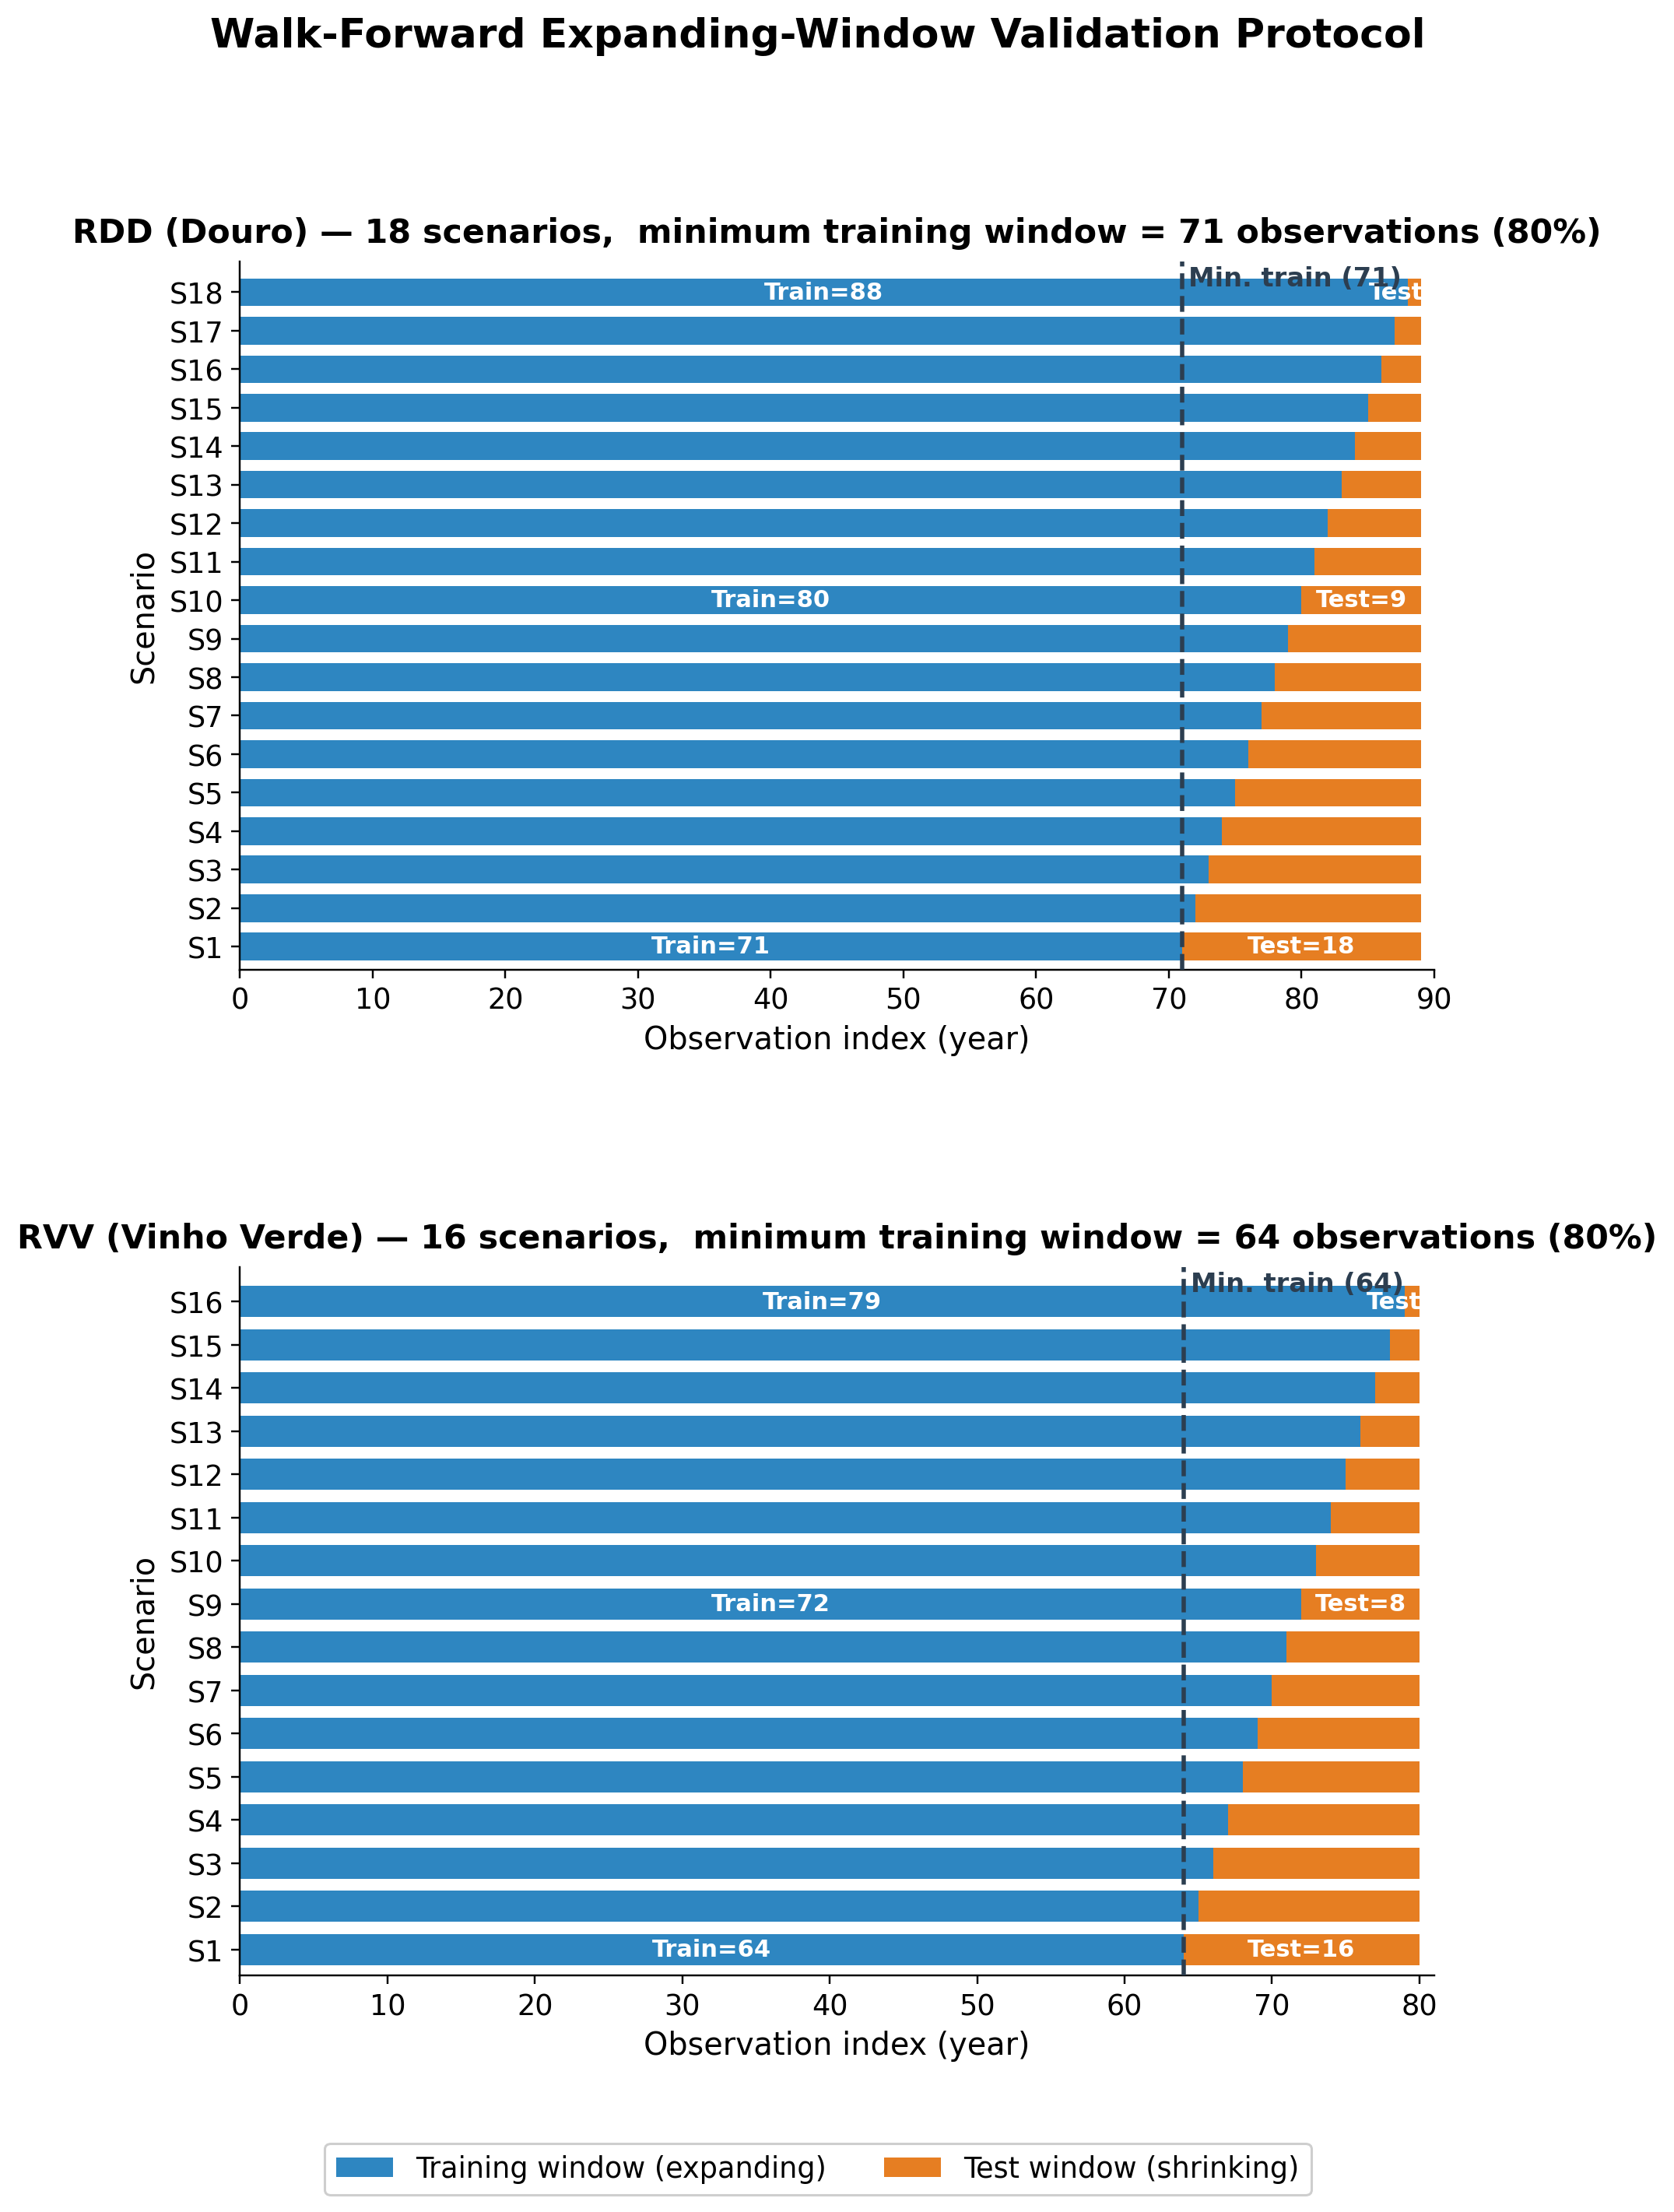
\includegraphics[width=\textwidth]{figures/fig_ch3_walkforward.png}
  \caption{Walk-forward expanding-window validation for RDD (18 scenarios, top) and RVV (16 scenarios, bottom).}
  \label{fig:ch3_walkforward}
\end{figure}


\section{Baseline Models}\label{sec:baseline_models}

\textbf{Naive\_Median: }predicts the median of the training-set residuals for every test year, equivalent to predicting that every test year will be exactly on trend. Minimises MAE among all constant predictors.

\textbf{Naive (last value): }predicts the most recently observed production value, corresponding to a random-walk assumption.

\textbf{Naive\_MA (moving average): }predicts the mean of the three most recent training observations in original units.

\textbf{Decision Tree (CART): }a CART regressor included as a non-rule-based ML comparator. Unlike the rule-learning algorithms, CART partitions the feature space using recursive binary splits that minimise squared error at each node, producing a tree structure rather than an explicit IF-THEN rule list. It was included to test whether the interpretability constraint comes at a cost in predictive performance relative to a standard ML baseline. The tree was fitted with default Weka hyperparameters within each training fold, subject to the same walk-forward protocol as all other models.

The 17 models evaluated in the walk-forward experiment span three categories: four baselines and comparators (Naive\_Median, Naive, Naive\_MA, and Decision Tree), two standard rule learners (RIPPER and M5Rules), and 11 CarenR variants. The baselines serve as benchmarks against which rule-learning algorithms are assessed: Naive\_Median is the primary reference (it minimises MAE under a constant prediction), while Naive and Naive\_MA test whether any model adds value over simpler alternatives that ignore climate information entirely. Decision Tree is included as a non-rule-based ML comparator to isolate the contribution of rule structure. The 11 CarenR variants all use the same distributional subgroup discovery algorithm but differ in how features are pre-selected within each training fold, enabling a systematic sensitivity analysis of this design choice. Table~\ref{tab:ch3a_4} lists all 17 models; Table~\ref{tab:ch3a_3} details the feature selection strategy distinguishing each of the 11 CarenR variants.

\begin{table}[htbp]
  \centering
  \caption{Complete set of 17 models evaluated in the walk-forward validation.}\label{tab:ch3a_4}
  \small
  \begin{adjustbox}{max width=\textwidth}
    \begin{tabularx}{\textwidth}{>{\ttfamily}p{5cm} p{2.8cm} X}
    \toprule
    \normalfont\textbf{Model} & \textbf{Type} & \textbf{Feature selection / distinguishing design choice} \\
    \midrule
    Naive\_Median        & Baseline       & Predicts training-set median residual (primary baseline) \\[3pt]
    Naive                & Baseline       & Predicts most recent observed value (random-walk) \\[3pt]
    Naive\_MA            & Baseline       & Predicts mean of 3 most recent training observations \\[3pt]
    Decision Tree        & ML comparator  & CART regressor on all 59 features; recursive binary splits \\[3pt]
    RIPPER               & Rule learner   & Classification rules on tertile-discretised residuals \\[3pt]
    M5Rules              & Rule learner   & Piecewise linear regression rules \\[3pt]
    CarenR\_Dist         & CarenR variant & All 59 features; default minimum support \\[3pt]
    CarenR\_Dist\_FS     & CarenR variant & Top-$N$ features by $|$Pearson correlation$|$ with target \\[3pt]
    CarenR\_Dist\_Thresh & CarenR variant & Features with $|$correlation$| \geq 0.30$ \\[3pt]
    CarenR\_Dist\_Sup    & CarenR variant & All 59 features; higher minimum support (broader rules) \\[3pt]
    CarenR\_Dist\_Sup\_Thresh & CarenR variant & Correlation threshold + higher minimum support \\[3pt]
    CarenR\_Dist\_Eta2   & CarenR variant & Top-$N$ features by $\eta^2$ (ANOVA on discretised bins) \\[3pt]
    CarenR\_Dist\_Lag    & CarenR variant & Sup\_Thresh config + lagged production residuals \\[3pt]
    CarenR\_Dist\_Conf   & CarenR variant & Sup\_Thresh config; confidence-weighted by $-\log(p\text{-value})$ \\[3pt]
    CarenR\_Dist\_Stack  & CarenR variant & Sup\_Thresh rules stacked with a lag regression step \\[3pt]
    CarenR\_Dist\_Sup\_FS & CarenR variant & Support-filtered + top-$N$ Pearson feature selection \\[3pt]
    CarenR\_Supervised   & CarenR variant & Per-fold supervised discretisation (cut-points maximise residual separation) \\
    \bottomrule
  \end{tabularx}
  \end{adjustbox}

\end{table}

\begin{table}[htbp]
  \centering
  \caption{CarenR variant families and their feature selection strategies.}\label{tab:ch3a_3}
  \small
  \begin{adjustbox}{max width=\textwidth}
    \begin{tabularx}{\textwidth}{>{\ttfamily}p{5cm} p{3.5cm} X p{3cm}}
    \toprule
    \normalfont\textbf{Variant} & \textbf{Feature selector} & \textbf{Selection criterion} & \textbf{Notes} \\
    \midrule
    CarenR\_Dist
      & None
      & All 59 features
      & Widest search; most risk of spurious rules \\[4pt]
    CarenR\_Dist\_FS
      & Pearson $|r|$, top-$N$
      & Retain above-median $|r|$ features
      & Most common baseline variant \\[4pt]
    CarenR\_Dist\_Eta2
      & $\eta^2$ (ANOVA effect size)
      & Bin-wise ANOVA $\eta^2$ with response
      & Best for RDD; captures non-linear association \\[4pt]
    CarenR\_Dist\_Sup\_FS
      & Pearson + support $\geq 20\%$
      & Conservative: $|r|$ + minimum bin coverage
      & Most stable across both regions \\[4pt]
    CarenR\_Dist\_Thresh
      & Pearson hard threshold
      & $|r| \geq 0.30$
      & Reduces feature set aggressively \\[4pt]
    CarenR\_Dist\_Sup
      & Pearson + support filter
      & $|r|$ + support filter (less strict than Sup\_FS)
      & Intermediate conservatism \\[4pt]
    CarenR\_Dist\_Lag
      & ACF-based lag features
      & Augment set with autocorrelated lags
      & Tests carryover temporal effects \\[4pt]
    CarenR\_Dist\_Conf
      & Confidence-weighted prediction
      & Weight rules by $1 - p$-value
      & Stronger rules get more prediction weight \\[4pt]
    CarenR\_Dist\_Stack
      & Two-stage stacking
      & CarenR residuals as second-stage input
      & Tests whether stacking adds value \\[4pt]
    CarenR\_Dist\_Sup\_Thresh
      & Pearson threshold + support filter
      & $|r| \geq 0.30$ + minimum bin coverage
      & Threshold and support combined; base for Lag, Conf, Stack variants \\[4pt]
    CarenR\_Supervised
      & Per-fold supervised bins
      & Maximise between-group residual SS (greedy 1D splits)
      & Evaluates target leakage from discretisation \\
    \bottomrule
  \end{tabularx}
  \end{adjustbox}

\end{table}


\section{Evaluation Metric}\label{sec:evaluation_metric}

The primary evaluation metric is scenario-size-weighted MAE on the original production scale (mhl):

\begin{equation}
  \text{Weighted MAE} = \frac{\sum_{s} n_s \times \text{MAE}_s}{\sum_{s} n_s}
  \label{eq:wmae}
\end{equation}

where $n_s$ is the number of test observations in scenario $s$. This weighting gives more influence to scenarios with larger test sets, which in the expanding-window design are the early scenarios with shorter training histories. Statistical significance of model differences was assessed using the Wilcoxon signed-rank test applied to per-scenario MAE pairs; the post-hoc era-balanced analysis used a binomial sign test (Section~\ref{sec:statistical_tests}).


\section{Software and Reproducibility}\label{sec:software_and_reproducibility}

The full pipeline was implemented in R (version 4.x). CarenR was run via the caren R package. RIPPER and M5Rules were run via RWeka, providing a JVM bridge to Weka 3.8. The pipeline is controlled by a master runner script (run\_all\_pipelines.R) that sequences data preparation, rule discovery, walk-forward validation, rule interpretation, and output generation. All detrending parameters and model hyperparameters are centralised in a configuration file (utils/config.R) to ensure reproducibility.


% ===== CONTINUATION =====


\subsection{Prediction Aggregation: Combining Multiple Firing Rules}\label{sub:prediction_aggregation_combining_multiple}

When multiple rules fire for a given test observation, their individual predictions must be aggregated into a single point estimate. Most CarenR variants use support-weighted aggregation; a small number use confidence weighting or equal weighting as alternatives. The primary source of divergence across the 11 variants is the feature selection strategy, not the aggregation mechanism. The general prediction formula for a test observation $x$ is:

where the sum is over all rules $i$ that fire for observation $x$ (i.e. all conditions of rule $i$ are satisfied by $x$), $m_i$ is the median residual of the training observations covered by rule $i$, and $w_i(x)$ is the weight assigned to rule $i$ for observation $x$. The weight definition distinguishes the variants.

Note on notation: $m_i$ denotes the median residual of the training observations in the subgroup defined by rule $i$. The tilde notation (˜) is used throughout to distinguish the median from the mean ($\mu$), following the convention that $\mu$ denotes a population mean and $m$ denotes a sample median.

\begin{table}[htbp]
  \centering
  \caption{Prediction aggregation formulas for the three CarenR variant families.}\label{tab:ch3b_1}
  \small
  \begin{adjustbox}{max width=\textwidth}
    \begin{tabularx}{\textwidth}{p{3.5cm} p{2.2cm} p{2.8cm} X}
    \toprule
    \textbf{Variant family} & \textbf{Weight $w_i(x)$} & \textbf{Formula} & \textbf{Rationale} \\
    \midrule
    Base (\texttt{Dist}, \texttt{FS}, \texttt{Eta2}, \texttt{Sup\_FS}, \texttt{Thresh}, \texttt{Lag})
      & Support of rule $i$
      & $w_i = s_i$ (fraction of training obs.\ covered)
      & Rules with higher coverage are weighted more — they represent more stable, generalisable patterns. A rule covering 28\% of years gets ${\approx}2\times$ the weight of one covering 15\%. \\[6pt]
    Confidence-weighted (\texttt{CarenR\_Dist\_Conf})
      & Confidence of rule $i$
      & $w_i = 1 - p_i$ (where $p_i$ is the KS $p$-value)
      & Rules with stronger statistical significance are weighted more. A rule with $p=0.004$ gets weight 0.996; a rule with $p=0.09$ gets weight 0.91. Prioritises statistical robustness over coverage. \\[6pt]
    Stacking (\texttt{CarenR\_Dist\_Stack})
      & Second-stage model weight
      & $w_i$ from a second-stage linear model fitted on rule predictions
      & Residuals from first-stage CarenR predictions are used as input to a second-stage model. Equivalent to learning an optimal linear combination of rule predictions on the training set. \\
    \bottomrule
  \end{tabularx}
  \end{adjustbox}

\end{table}


For the default support-weighted case (used by the majority of variants), the full prediction formula for test year $t$ is:

where $F(t) = \{i : \text{all conditions of rule } i \text{ are satisfied by features of year } t\}$ is the set of firing rules, $s_i \in [0.15, 1.0]$ is the support fraction of rule $i$, $m_i$ is the median detrended production residual among training observations covered by rule $i$, and $\mathrm{median}(r_1, \ldots, r_n)$ is the training-set median residual (the Naive\_Median prediction, used as fallback when no rules fire).

A worked example illustrates the formula. Suppose test year 2015 has the following feature values: wet days post-flowering = 1.2 days, soil water pre-harvest = 89 mm, heat days post-flowering = 0.4 days. Three rules fire:

\begin{table}[htbp]
  \centering
  \caption{Worked example of the support-weighted prediction formula.}\label{tab:ch3b_2}
  \small
  \begin{adjustbox}{max width=\textwidth}
    \begin{tabularx}{\textwidth}{p{1.2cm} X p{2.5cm} p{1.8cm} p{3cm}}
    \toprule
    \textbf{Rule} & \textbf{Conditions matched} & \textbf{Subgroup median $\tilde{m}_i$} & \textbf{Support $s_i$} & \textbf{Weighted contribution $s_i \cdot \tilde{m}_i$} \\
    \midrule
    Rule 1
      & Wet days post-flowering $\in [0, 3.3\,\text{d}]$\newline Wet days post-maturity $\in [0, 3.5\,\text{d}]$
      & $+121$ mhl & 0.281 & 34.00 \\[6pt]
    Rule 5
      & Wet days post-flowering $\in [0, 3.3\,\text{d}]$\newline Heat days pre-maturity $\in [0, 3.7\,\text{d}]$
      & $+115$ mhl & 0.247 & 28.41 \\[6pt]
    Rule 7
      & Wet days post-flowering $\in [0, 3.3\,\text{d}]$\newline Soil water pre-harvest $\in [74, 231\,\text{mm}]$\newline Heat days pre-maturity $\in [0, 3.7\,\text{d}]$
      & $+115$ mhl & 0.213 & 24.50 \\[6pt]
    \midrule
    Sum   & & & $\sum s_i = 0.741$ & $\sum s_i \tilde{m}_i = 86.91$ \\[4pt]
    \textbf{Prediction} & \multicolumn{4}{l}{$\hat{y} = 86.91\,/\,0.741 = +117.3$ mhl} \\
    \bottomrule
  \end{tabularx}
  \end{adjustbox}

\end{table}


The predicted residual (+117.3 mhl) is then re-trended by adding the linear trend value projected to 2015 to produce the final production estimate in mhl. This re-trending step ensures the prediction is on the original scale and directly comparable to the actual production value for the MAE computation.

\textbf{Why support weighting rather than equal weighting? }Equal weighting would give every firing rule the same influence regardless of how broadly applicable it is. A rule covering 15\% of training years (the minimum support threshold adopted in this thesis) represents a pattern seen in roughly 13 years out of 89; a rule covering 28\% of years was observed in approximately 25 years. Giving equal weight to both would over-represent narrow, potentially less stable patterns. Support weighting is a principled way to account for statistical reliability without fully discarding less-common rules; they still contribute, but proportionally to their historical recurrence.

\textbf{The confidence-weighted variant (CarenR\_Dist\_Conf) }uses $1-p_i$ as the weight, giving more influence to rules whose subgroup distribution is most statistically distinct from the global distribution. In theory, this should favour the most reliable patterns; in practice, it performs comparably to support weighting (RDD rank 6, RVV rank 3 in Table~\ref{tab:ch5a_1}), suggesting that KS p-value and support are correlated enough that both approaches identify the same rules as most important.

\textbf{When exactly one rule fires, }the formula simplifies to $\hat{y}(t) = m_i$, the prediction is simply the median residual of the matching subgroup, independent of support (which cancels). The support weighting only has an effect when two or more rules fire simultaneously, resolving conflicts by favouring more broadly applicable rules.


% ===== CONTINUATION =====


\section{Formal Stationarity Testing}\label{sec:formal_stationarity_testing}

The need for detrending is not merely heuristic: both production series exhibit statistically significant non-stationarity in their raw form, formally confirmed by two complementary tests. The Augmented Dickey-Fuller (ADF) test uses the null hypothesis that a unit root is present (non-stationary); rejection at $\alpha$ = 0.05 indicates stationarity. The KPSS (Kwiatkowski-Phillips-Schmidt-Shin) test reverses this logic, using the null hypothesis of stationarity; rejection indicates non-stationarity. Applying both tests provides a more robust assessment than either test alone, since ADF has low power against near-unit-root processes and KPSS is sensitive to long-run variance estimation.

Table~\ref{tab:ch3c_1} reports the test results for the raw production series and the linear detrended residuals for both regions.

\begin{table}[htbp]
  \centering
  \caption{Stationarity test results. ADF H$_0$: unit root present.}\label{tab:ch3c_1}
  \small
  \setlength{\tabcolsep}{4pt}
  \begin{adjustbox}{max width=\textwidth}
    \begin{tabularx}{\textwidth}{p{0.9cm}|p{2.2cm}|p{1.3cm}|p{1.3cm}|p{2cm}|p{1.3cm}|p{1.3cm}|X}
  \toprule
  Region & Series & ADF statistic & ADF p-value & Verdict & KPSS statistic & KPSS p-value & Verdict \\
  \midrule
  RDD & Raw (Wine\_mhl) & -1.800 & 0.381 & Non-stationary
(unit root) & 0.134 & 0.071 & Borderline stationary
around trend \\
  RDD & Linear detrended
residuals & -8.520 & <0.001 *** & Stationary $\checkmark$ & 0.134 & 0.100 & Stationary $\checkmark$ \\
  RVV & Raw (Wine\_mhl) & -0.490 & 0.894 & Non-stationary
(unit root) & 0.332 & 0.010 ** & Non-stationary
(rejects stationarity
around trend) \\
  RVV & Linear detrended
residuals & -1.817 & 0.372 & Non-stationary
(unit root remains) & 0.332 & 0.100 & Stationary $\checkmark$
(level stationarity) \\
  \bottomrule
\end{tabularx}
  \end{adjustbox}

\end{table}


The results have three important implications for the methodological choices made in this thesis.

\textbf{Implication 1: Detrending is formally justified for both regions. }Both raw series fail the ADF test (p = 0.38 for RDD, p = 0.89 for RVV), confirming that unit roots cannot be rejected in either series. The linear trend slopes are both highly statistically significant (p < 0.0001), confirming that the observed trends are not artefacts of sampling variability. Applying machine learning models to the raw series without detrending would violate the stationarity assumptions implicit in cross-sectional feature-based modelling and would confound climate effects with structural level changes.

\textbf{Implication 2: Linear detrending achieves full stationarity in RDD but only partial stationarity in RVV. }After linear detrending, the RDD residuals pass both the ADF test (p < 0.001) and the KPSS test (p = 0.10), confirming stationarity by both criteria. The RVV residuals pass the KPSS level-stationarity test (p = 0.10) but fail the ADF test (p = 0.37), indicating that a unit root cannot be rejected even after removing the linear trend. This is formal statistical evidence that the RVV structural change, the sharp non-linear decline associated with EU accession and industry restructuring, is not fully captured by a linear trend. Persistent non-stationarity in the RVV residuals means that the era-composition effects observed in the walk-forward evaluation (Section~\ref{sec:era_composition_and_perscenario_rvv}) have a formal statistical basis: the residuals themselves are non-stationary, which means rules discovered in early training windows may not generalise to later test windows.

\textbf{Implication 3: The mixed RVV result formally motivates LOESS detrending as a more flexible alternative. }The fact that RVV residuals pass KPSS but fail ADF after linear detrending confirms that the linear trend removes the long-run structural level but not all persistent structure. A more flexible detrending (LOESS) would in principle resolve this residual non-stationarity. The LOESS sensitivity analysis (Section~\ref{sec:detrend_sensitivity_analysis_loess}) demonstrates that LOESS does reduce the Naive\_Median baseline substantially for RVV, consistent with reducing the residual non-stationarity. However, it simultaneously removes the climate signal required for rule induction, a direct empirical manifestation of the Decision 1 / Decision 2 trade-off formalised in Section~\ref{sec:detrending_and_the_twodecision}.

The stationarity test results therefore serve as formal grounding for three methodological choices: (1) the decision to detrend rather than model raw production values; (2) the acknowledgement that linear detrending is imperfect for RVV and that some residual non-stationarity remains; and (3) the decision to retain linear detrending despite this imperfection, because the alternative (LOESS) resolves the non-stationarity at the cost of eliminating the climate signal that is the thesis's primary object of study.



\section{Data Sources}\label{sec:data_sources}

The datasets for both regions originate from two independent source streams that were joined at the annual level.


\subsection{Meteorological Data}\label{sub:meteorological_data}

Daily meteorological records for the Douro region were sourced from the BCM base climate files maintained by the University of Porto's viticulture research group (Professor Mário Cunha). The source files (BCM\_base\_RDD.xls, BCM\_base\_RVV.xls) contain one row per calendar day from 1933-01-01 to 2022-12-31 for RDD (32,842 daily records) and from 1941-01-01 to 2022-11-13 for RVV (29,902 daily records). Each daily record contains the following primary meteorological variables:

\begin{table}[htbp]
  \centering
  \caption{Primary daily meteorological variables in the raw source files.}\label{tab:ch3d_1}
  \small
  \begin{adjustbox}{max width=\textwidth}
    \begin{tabularx}{\textwidth}{llX}
    \toprule
    \textbf{Variable} & \textbf{Description} & \textbf{Unit} \\
    \midrule
    Tmax & Daily maximum temperature & $^\circ$C \\
    Tmin & Daily minimum temperature & $^\circ$C \\
    Tmed & Daily mean temperature & $^\circ$C \\
    Rain & Daily total rainfall & mm \\
    Sm   & Soil water availability (model-derived) & mm \\
    Iaf  & Leaf Area Index (phenological model) & m$^2$/m$^2$ \\
    Eto  & Reference evapotranspiration & mm \\
    \bottomrule
  \end{tabularx}
  \end{adjustbox}

\end{table}


The soil water availability (Sm) and Leaf Area Index (Iaf) values are not direct measurements but model-derived estimates produced by the Vineyard Soil Irrigation Model (VSIM) calibrated to each region's soil and vine characteristics by Professor Cunha's group over decades of field work \citep{Cunha2016}. These modelled variables are critical for the analysis: Sm represents the balance between precipitation, evapotranspiration, and soil water-holding capacity integrated daily, while IAF represents vine canopy development as a continuous daily estimate anchored to the vine's phenological state.

In Stage 1 of the pipeline (script: 1\_data\_preparation\_stage\_1.R), five binary/threshold indicator variables were derived from the pre-processed daily records provided by Professor Cunha's group:

\begin{table}[htbp]
  \centering
  \caption{Binary threshold indicators derived from raw daily meteorological variables.}\label{tab:ch3d_2}
  \small
  \begin{adjustbox}{max width=\textwidth}
    \begin{tabularx}{\textwidth}{p{3cm} p{3.5cm} X}
    \toprule
    \textbf{Derived indicator} & \textbf{Condition} & \textbf{Agronomic meaning} \\
    \midrule
    \texttt{R>0.1}    & Rain $> 0.1$ mm                       & Wet day indicator (trace rainfall) \\
    \texttt{Tmed<15}  & Tmed $< 15^\circ$C                    & Cold day, impairs flowering and fruit set \\
    \texttt{Tmax>35}  & Tmax $> 35^\circ$C                    & Heat-stress day, causes flower abortion, accelerates ripening \\
    \texttt{Tmin<0}   & Tmin $< 0^\circ$C                     & Frost day, potential bud and shoot damage \\
    \texttt{Sm<1.5Wp} & Sm $< 1.5 \times$ wilting point       & Severe soil water stress, below vine survival threshold \\
    \texttt{Sm>0.9Fc} & Sm $> 0.9 \times$ field capacity      & Near-saturation, promotes disease, excessive vigour \\
    \bottomrule
  \end{tabularx}
  \end{adjustbox}

\end{table}


The resulting Stage 1 output is a clean daily dataset with 17 columns per region (dataPrep\_meteo\_rdd.csv, dataPrep\_meteo\_rvv.csv) spanning the full time horizon.


\subsection{Phenology and Production Data}\label{sub:phenology_and_production_data}

Annual wine production records and vine phenological dates were sourced from the Pheno\_Prd source files maintained by the same research group (Pheno\_Prd\_1933\_2022\_recente.xlsx for RDD; equivalent for RVV). Each annual record contains:

\begin{table}[htbp]
  \centering
  \caption{Annual phenology and production variables.}\label{tab:ch3d_3}
  \small
  \begin{adjustbox}{max width=\textwidth}
    \begin{tabularx}{\textwidth}{l|X}
  \toprule
  Variable & Description \\
  \midrule
  Wine\_mhl & Annual regional wine production (thousands of hectolitres) \\
  DOY\_BB & Day of Year of Bud Break, start of vegetative growth \\
  DOY\_Fl & Day of Year of Flowering, critical fruit-set window \\
  DOY\_sM & Day of Year of Start of Maturity (veraison), berry ripening begins \\
  DOY\_Fs & Day of Year of Fruit Set, end of berry cell division \\
  DOY\_Hv & Day of Year of Harvest, end of growing season \\
  \bottomrule
\end{tabularx}
  \end{adjustbox}

\end{table}


The phenological dates (DOY\_BB through DOY\_Hv) are derived from the STICS (Simulateur mulTIdisciplinaire pour les Cultures Standard) phenological sub-model and represent the average calendar date of each key event across the regional vine population for each year. These dates vary by 2--4 weeks across years for each stage, reflecting the sensitivity of vine phenology to temperature, warmer springs advance flowering and harvest, cooler springs delay them. The variability in these anchor dates is what makes phenology-based windowing more informative than fixed calendar windows: a feature computed as ``the 20 days before Harvest'' adapts to the actual harvest date of each year rather than always covering, say, the first three weeks of September.

The production series for RDD spans 1933--2022 (90 observations), but the feature construction starts at 1934 to allow for previous-year (y0) features, leaving 89 usable observations. For RVV, the series spans 1942--2021 with 80 usable observations. The production values show the structural trajectories described in Chapter~\ref{ch:literature_review}: RDD production ranging from 518 to 1,961 mhl with a mean of 1,116 mhl and an upward trend; RVV production ranging from 494 to 3,443 mhl with a mean of 1,621 mhl and a sharp downward trend since the 1960s.


\section{Feature Engineering: From Daily Records to Annual Features}\label{sec:feature_engineering_from_daily}

The core methodological contribution of the data pipeline is the transformation from 32,842 (RDD) and 29,902 (RVV) daily records into 59 annual agroclimatic features per region. This transformation is performed by script 2\_features\_creation.R and is anchored entirely on the phenological dates for each year. For each year y1, each combination of (meteorological variable $\times$ phenological anchor $\times$ window position $\times$ window width $\times$ year offset) defines one feature.


\subsection{Feature Naming Convention}\label{sub:feature_naming_convention}

All 59 features follow a systematic naming convention that encodes all relevant information about how the feature was computed:

{variable}\_{stage}\_{year}\_{position}{width}

where:

\begin{table}[htbp]
  \centering
  \caption{Feature naming convention components.}\label{tab:ch3d_4}
  \small
  \begin{adjustbox}{max width=\textwidth}
    \begin{tabularx}{\textwidth}{p{1.8cm}|X|p{4.5cm}}
  \toprule
  \textbf{Component} & \textbf{Options} & \textbf{Meaning} \\
  \midrule
  \texttt{variable} & \texttt{tm, tn, swa, iaf, rf, days.rf, sw.less.15wp, sw.above.09fc, days.maxTemp.above.35, tm.days.less.15, days.minTemp.less.0} & Meteorological quantity aggregated \\[4pt]
  \texttt{stage} & \texttt{bb} (Bud Break), \texttt{fl} (Flowering), \texttt{sM} (Start Maturity), \texttt{hv} (Harvest) & Phenological anchor point \\[4pt]
  \texttt{year} & \texttt{y1} (current year), \texttt{y0} (previous year) & Growing season reference \\[4pt]
  \texttt{position} & \texttt{c} (centred), \texttt{b} (before), \texttt{a} (after) & Window position relative to stage \\[4pt]
  \texttt{width} & \texttt{5, 10, 15, 20, 30} (days) & Aggregation window width \\
  \bottomrule
\end{tabularx}
  \end{adjustbox}

\end{table}


For example: swa\_hv\_y1\_b20 = soil water availability (swa), in the 20 days BEFORE (b20) Harvest (hv), in the current year (y1). tm\_fl\_y0\_b10 = mean temperature (tm), in the 10 days BEFORE (b10) Flowering (fl), in the PREVIOUS year (y0). iaf\_fl\_y1\_a10 = Leaf Area Index (iaf), in the 10 days AFTER (a10) Flowering (fl), in the current year (y1).


\subsection{Feature Groups and Counts}\label{sub:feature_groups_and_counts}

Table~\ref{tab:ch3d_5} summarises the 59 features by variable family and their counts. The distribution reflects the relative importance of different variable types in the viticulture literature: mean temperature (tm) and minimum temperature (tn) variables are most numerous because temperature governs nearly every phenological process; soil water and LAI variables are next because they are the primary within-season stress indicators; rainfall and heat/cold day counts complete the picture.

\begin{table}[htbp]
  \centering
  \caption{Feature groups, counts, and agronomic meanings. Total: 59 features per region.}\label{tab:ch3d_5}
  \small
  \begin{adjustbox}{max width=\textwidth}
    \begin{tabularx}{\textwidth}{X|p{4cm}|p{1cm}|p{4.5cm}}
  \toprule
  \textbf{Variable family} & \textbf{Symbol} & \textbf{N} & \textbf{What it measures} \\
  \midrule
  Mean daily temperature & tm & 12 & Average thermal conditions at key phenological windows \\
  Leaf Area Index & iaf & 10 & Vine canopy development, proxy for vegetative vigour \\
  Soil water deficit days & sw.less.15wp & 8 & Days when soil water < 1.5$\times$ wilting point, severe stress \\
  Rainfall event count & days.rf.above.1mm & 6 & Number of days with rainfall > 1 mm, disease pressure proxy \\
  Soil water availability & swa & 5 & Absolute soil water balance at harvest and flowering windows \\
  Soil saturation days & sw.above.09fc & 4 & Days when soil water > 90\% field capacity, excess moisture \\
  Heat stress days (Tmax > 35$^\circ$C) & days.maxTemp.above.35 / days.tempMax.above.35 & 4 & Extreme heat events, flower abortion and thermal damage \\
  Rainfall sum & rf & 3 & Total precipitation at harvest and flowering windows \\
  Cold days (Tmed < 15$^\circ$C) & tm.days.less.15 & 2 & Cool days impairing pollination and fruit set \\
  Frost days (Tmin < 0$^\circ$C) & days.minTemp.less.0 & 2 & Frost events, bud and shoot damage risk \\
  Minimum temperature & tn & 1 & Night temperature at harvest, berry quality proxy \\
  Previous-year soil water & y0 variants of swa/sw & 2 & Carry-over water stress from prior season \\
  \bottomrule
\end{tabularx}
  \end{adjustbox}

\end{table}



\subsection{Current-Year vs Previous-Year Features}\label{sub:currentyear_vs_previousyear_features}

A key design decision in the feature engineering was the inclusion of previous-year (y0) features alongside current-year (y1) features. As discussed in Section~\ref{sec:grapevine_yield_formation}, vine physiology has a two-year temporal structure: inflorescence primordia that determine current-year bunch number are formed in the prior growing season, and vine carbohydrate reserves that determine shoot vigour are accumulated during the prior year's harvest-to-dormancy period. Failing to include prior-year features would miss this carry-over mechanism entirely.

In the final feature matrix, 15 of the 59 features (25\%) use y0 (previous-year) anchors. The most agronomically motivated y0 features are:

\textbf{tm\_fl\_y0\_b10 }(mean temperature in the 10 days before previous-year flowering): captures the thermal conditions governing inflorescence primordia formation in the prior season, the mechanism that determines current-year bunch potential.

\textbf{tm\_bb\_y0\_a30 }(mean temperature in the 30 days after previous-year bud break): captures the early-season thermal conditions that initiate the prior year's vegetative growth phase, influencing vine carbohydrate allocation.

\textbf{tm\_sm\_y0\_a20 }(mean temperature in the 20 days after previous-year start of maturity): captures the heat load during the prior year's ripening phase, which governs both berry quality in the prior year and the vine's thermal stress exposure at the end of the growing season.

\textbf{sw.above.09fc\_fl\_y0\_a20 }(soil saturation days in the 20 days after previous-year flowering): captures prior-year excess soil moisture during flowering, the carry-over mechanism identified in RVV CarenR Rule 2 (see Section~\ref{sub:vinho_verde_rvv_top}).


\subsection{Feature Discretisation for CarenR}\label{sub:feature_discretisation_for_carenr}

The continuous feature matrix (dataPrep\_cont\_dataset\_*.csv, 59 columns $\times$ 89/80 rows) is used directly by M5Rules and RIPPER, which perform their own internal threshold finding. For CarenR, a separate discretised version of the dataset (dataPrep\_dis\_rule\_dataset\_*.csv) is produced by script 2\_features\_creation.R using equal-frequency binning into four quartile intervals. Each feature is independently divided into four bins, each containing approximately 25\% of the training observations, with the boundaries represented as interval notation (e.g. [18.3|22.4] for the bin from 18.3$^\circ$C to 22.4$^\circ$C).

The equal-frequency choice, rather than equal-width or domain-knowledge-based breakpoints, ensures that each bin is populated by a comparable number of observations. This is important for the KS test used by CarenR: a bin with only two or three observations would produce an unreliable distributional comparison regardless of its meteorological significance. In the walk-forward scenarios, the bin boundaries are re-estimated within each training fold, ensuring that the discretisation reflects the distribution of climate conditions actually observed in the training period, not the full historical record that would be unknowable at prediction time.


\section{Data Pipeline Summary}\label{sec:data_pipeline_summary}

The pipeline was implemented as a sequence of seven R scripts coordinated by a master runner (run\_all\_pipelines.R), with all intermediate datasets written to disk at each stage to allow inspection and validation. The complete stage-by-stage breakdown is given in Table~\ref{tab:ch3d_6} and the fixed configuration parameters in Table~\ref{tab:ch3d_7}, both in Appendix~\ref{app:exploratory_data_analysis}. Figure~\ref{fig:ch3_pipeline} in the same appendix shows the full pipeline schematically.

